\scanpage{205}

\figure{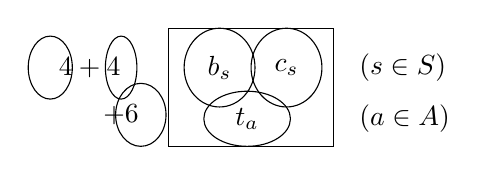
\begin{tikzpicture}
\node at (0,0) {$4+4$};\node at (.4,-.6) {$+6$};
\draw (-.5,0) ellipse(.28 and .4);\draw (.4,0) ellipse(.2 and .4);\draw (.65,-.6) ellipse(.32 and .4);
\draw (1,-1)--(1, .5)--(3.1,.5)--(3.1,-1)--cycle;
\node at (1.65,0) {$b_s$};\node at (2.5,0) {$c_s$};\node at (2,-.65) {$t_a$};
\draw (1.65,0) ellipse(.45 and .5);\draw (2.5,0) ellipse(.45 and .5);\draw (2,-.65) ellipse(.55 and .35);
\node[right] at (3.3,0) {$(s\in S)$};\node[right] at (3.3,-.65) {$(a\in A)$};
\end{tikzpicture}}
avec $b_s=b_{\bar s}$, $c_s=c_{\bar s}$, $\unsure{b_a|t_a}=t_{\bar a}$.

\figure{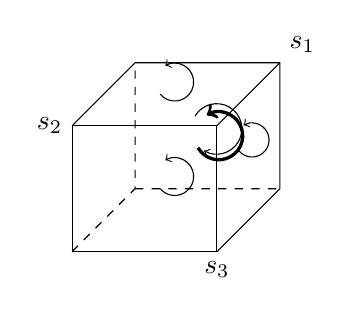
\begin{tikzpicture}[scale=.8]
\draw (0,0)--(0,2)--(2.3,2)--(2.3,0)--cycle;
\draw (0,2)--(1,3)--(3.3,3)--(3.3,1)--(2.3,0) (2.3,2)--(3.3,3);
\draw[dashed] (0,0)--(1,1)--(1,3) (1,1)--(3.3,1);
\node[above right] at (3.3,3) {$s_1$};\node[left] at (0,2) {$s_2$};\node[below] at (2.3,0) {$s_3$};
\draw[->] (1.4,2.5) arc(220:480:.3);
\draw[->] (1.4,1) arc(220:480:.3);
\draw[->] (2.65,1.6) arc(220:480:.27);
\draw[->] (1.95,2.15) arc(150:-120:.4);
\draw[->,very thick] (2,1.65) arc(210:480:.38);
\end{tikzpicture}}
Si $\delta(s)\inserted{\in I}$ est la diagonale qui passe par $s$, on a
\[b_s=\operatorname{Tr}X_s\qquad c_s=\det X_s\]
Si $\delta(a)\in\unsure{\mathcal P|P}_2(I)$ est l'une des deux diagonales qui passent par les
\deleted{\unsure{sommets}} de $a$, on a
\[t_a=\operatorname{Tr}X_iX_j\inserted{=\operatorname{Tr}X_jX_i}
\quad\text{si }\delta(a)=\{i,j\}\]

\figure{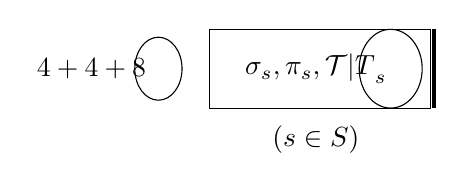
\begin{tikzpicture}
\node at (0,0) {$4+4+8$};\draw (.85,0) ellipse(.3 and .4);
\draw (1.5,-.5) rectangle (4.3,.5);\draw[very thick] (4.35,-.5)--(4.35,.5);
\node at (2.85,0) {$\sigma_s,\pi_s,\unsure{\mathcal T|T}_s$};\draw (3.8,0) ellipse(.4 and .5);
\node at (2.85,-.9) {$(s\in S)$};\end{tikzpicture}}
$s$ correspond à un triple $(i,j,k)$ à perm. circulaire près
\[\begin{aligned}
\mathcal T_s&=\operatorname{Tr}X_iX_jX_k
 =\operatorname{Tr}X_{\deleted{\unsure{i}}\inserted{j}}X_kX_i
 =\operatorname{Tr}X_kX_iX_j\\
\mathcal T_{\bar s}&=\operatorname{Tr}X_kX_jX_i
 =\operatorname{Tr}X_jX_iX_k=\operatorname{Tr}X_iX_kX_j .
\end{aligned}\]

\figure{\begin{tikzpicture}
\node[draw,ellipse] at (0,0) {$4+4$ relations};
\node at (2.2,0) {$(R_s)$};\node at (2.2,-.5) {$\underbrace{\phantom{R_s}}_{R_{\bar s}}$};
\node[draw,rectangle] at (5,0) {$\begin{aligned}
\sigma_s&=\sigma_{\bar s}=\mathcal T_s+\mathcal T_{\bar s}\\
\pi_s&=\unsure{\pi_{\bar s}|\sigma_{\bar s}}=\mathcal T_s\cdot\mathcal T_{\bar s}
\end{aligned}$};\end{tikzpicture}}
\[\begin{aligned}
\sigma_s=\sigma_{\bar s}&=b_it_{jk}+b_jt_{ki}+b_kt_{ij}-b_ib_jb_k\\
\deleted{\unsure{\sigma_s}}&=b_{s_1}t_{ss_1}+b_{s_2}\unsure{b_{ss_2}|t_{ss_2}}+b_{s_3}t_{ss_3}-b_{s_1}b_{s_2}b_{s_3}
\end{aligned}\]
où $s_1,s_2,s_3$ sont les sommets adjacents à $s$
\[\left\{\begin{aligned}
\pi_s=\pi_{\bar s}={}&t_{ss_1}t_{ss_2}t_{ss_3}
 +\deleted{(c_{s_1}t_{ss_1}^{\unsure{2}}+c_{s_2}t_{ss_2}^{\unsure{2}}+c_{s_3}t_{ss_3}^{\unsure{2}})}\\
&\inserted{+\bigl[c_{s_1}t_{ss_1}(t_{ss_1}-b_{s_2}b_{s_3})
 +c_{s_2}t_{ss_2}(t_{ss_2}-b_{s_3}b_{s_1})
 +c_{s_3}t_{ss_3}(t_{ss_3}-b_{s_1}b_{s_2})\bigr]}\\
&+(\unsure{b_{ss_1}^{2}|b_{s_1}^{2}}c_{ss_2}c_{ss_3}
 +\unsure{b_{ss_2}^{2}|b_{s_2}^{2}}c_{ss_3}c_{ss_1}
 +\unsure{b_{ss_3}^{2}|b_{s_3}^{2}}c_{ss_1}c_{ss_2})
\end{aligned}\right.\]

\figure{\begin{tikzpicture}
\node[draw,ellipse] at (0,0) {$6$};
\draw (1,-1.2)--(1,.5)--(2.1,.5)--(2.1,-.4)--(2.8,-.4)--(2.8,-1.2)--cycle;
\node[draw,ellipse] at (1.6,0) {$\mathcal T_f$};\node at (1.9,-.9) {$\sigma_a,\pi_a$};
\node[right] at (2.5,0) {$(f\in F)$};\node[right] at (3,-.9) {$(a\in A)$};\end{tikzpicture}}
Si $f$ correspond à la permutation circulaire $(i,j,k,l)$ de $I$, on a
\[\mathcal T_f=\operatorname{Tr}X_iX_jX_kX_l
 =\deleted{\unsure{\mathcal T_f=}}\operatorname{Tr}X_jX_kX_lX_i
 =\operatorname{Tr}X_kX_lX_iX_j=\operatorname{Tr}X_lX_iX_jX_k\]
Si $f,f'$ sont adjacentes le long d'une arête $a=(s,t)$

\figure{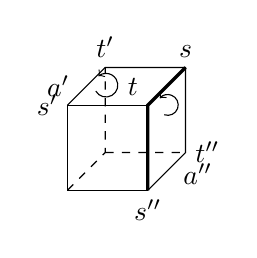
\begin{tikzpicture}[scale=.6]
\draw (0,0)--(0,1.8)--(1.7,1.8)--(1.7,0)--cycle;
\draw (0,1.8)--(.8,2.6)--(2.5,2.6)--(2.5,.8)--(1.7,0) (1.7,1.8)--(2.5,2.6);
\draw[dashed] (0,0)--(.8,.8)--(.8,2.6) (.8,.8)--(2.5,.8);
\draw[very thick] (1.7,0)--(1.7,1.8)--(2.5,2.6);
\node[above] at (2.5,2.6) {$s$};\node[above left] at (1.7,1.8) {$t$};
\node[left] at (0,1.8) {$s'$};\node[above] at (.8,2.6) {$t'$};
\node[below] at (1.7,0) {$s''$};\node[right] at (2.5,.8) {$t''$};
\node[right] at (2.25,.35) {$a''$};\node[left] at (.25,2.2) {$a'$};
\draw[->] (.6,2.1) arc(210:490:.25);\draw[->] (2.05,1.6) arc(250:500:.22);
\end{tikzpicture}}

\diagram{\begin{tikzcd}[ampersand replacement=\&, row sep=small,column sep=small]
f=(s,\arrow[d]\&t,\arrow[d]\&s'',\arrow[d]\&t'')\arrow[d]\&\quad f'=(t,\arrow[d]\&s,\arrow[d]\&t'',\arrow[d]\&s'')\arrow[d]\\
i\&j\&k\&l\&j\&i\&k\&l
\end{tikzcd}}
\deleted{\unsure{NB}} d'où
\[\mathcal T_f=\operatorname{Tr}X_iX_j(X_kX_l),\quad
\mathcal T_{f'}=\operatorname{Tr}X_jX_i(X_kX_l),\quad\text{on a}\]
\margin{204}
